\section{Research}\label{Section:Research}
Before development can begin, it is important to understand the problem and existing technologies that exist to combat it. This allows the developer to learn about what is currently missing and can be implemented for a superior system. A range of technologies also exist which simplify the development process and can be utilised to create an efficient solution rather than ``reinventing the wheel''. These technologies are researched and discussed with their benefits and costs so the developer can make an informed decision. Additionally, it is likely that previous research will have been conducted in the area and can provide guidance for design and implementation of the system.

\subsection{Existing Systems}
Several systems exist which have previously attempted to tackle the aforementioned problem. Unfortunately, all these systems only provide a partial solution and hence are incomplete. These systems, more often than not, come with drawbacks and also with a price in some cases. In order to develop a complete solution, which has potential in the market, it is necessary to study these existing solutions so one can identify where these systems are performing well and where they are lacking.

\subsubsection{Immobilise}
Immobilise, as stated on their website, helps combat the sale of stolen gadgets and valuable goods as well as help police identify the owners of recovered property \cite{Immobilise:Home}. The system has been around for over 11 years \cite{Immobilise:Home}. Immobilise can be used by members of the public and businesses to register their valued possessions or company assets, and exclusive to Immobilise all account holders registered items and ownership details are viewable on the police national property database \cite{Immobilise:Home}. In essence, users can sign-up to the site and then register their valuables and possessions on their profile. These items are stored in a database which is only available to the police for querying. The police is able to search the database and retrieve the details of the item as well as details of its owner when they come across stolen property. 

This system works well by allowing users to register their possessions at any time. The details are only visible to the user and the police which protects the users details. Unfortunately, the downfall of this system is that the police only checks items against this database once they have been recovered. This means that unless the police has raided a location containing stolen items, the item won’t be checked against the database. Additionally, individuals are unable to cross check items, when making purchases, using Immobilise. This limits the system and only benefits victims of theft rather than protecting more people from becoming victims.

\subsubsection{CheckMEND} \label{Section:CheckMEND}
CheckMEND is currently the world's largest source of used mobile phone and device history, including data from police, insurers, retailers and networks \cite{CheckMEND:Home}. CheckMEND comes from the early days of the Recipero Crime Reduction Ecosystem which was once know as the Mobile Equipment National Database, or M.E.N.D. for short and is essentially just checking M.E.N.D \cite{CheckMEND:Home}. The system offers services which allows individual users or organisations to check the history of a mobile phone or device but the results are not guaranteed. The results are provided in the form of a report which details the history of the device, if any is available.

The main advantage of CheckMEND is that it allows individual to generate reports about the history of a device, hence protecting potential buyers from being defrauded. Unfortunately, regardless of whether the check actually returns any results or not, every check carried out using CheckMEND comes with a price of tag \pounds1.99. If the CheckMEND report doesn't show any history for the device, this does not ensure that the history is clean, it just means that no history has been reported. Another limitation of this system is that it is restricted to only mobile phones and electronic devices with an IMEI or a serial number.

\subsubsection{Stolen-Bikes} \label{Section:Stolen-Bikes}
Stolen-Bikes is fundamentally similar to CheckMEND and Immobilise \cite{StolenBikes:Home}. It allows user to report a bike as stolen, without having to sign up for an account, using a simple form. To report a bike, the user simply provides the make, model, and other information about the bike which would help another person to identify it. The system allows the users to search for bikes reported as stolen by make, model, and various other attributes. Additionally, the user can also search for bikes reported as stolen in a specified area using postcode or area name.

This system provides a complete solution for bikes, however it is limited by the fact that it's only available for bikes. This allows the system to be very specific and allow users to query the data using a wide range of attributes. The map functionality allows users to view hotspots for bike theft. This means, if users know they are leaving their bike in a theft hotspot, users can be cautious and introduce more security measures or completely avoid leaving their bikes outdoor in the area.

\subsection{Technologies Used}\label{Section:Research_Technologies}
When developing a web application, it is important to explore the range of technologies already available in order to speed up the development process. For this reason, several third party technologies were used to provide some of the core functionality of the system. These technologies include but are not limited to jQuery, Laravel and Google Maps. In addition to the third party technologies, the latest web development technologies were also employed to provide the essential and basic functionality of a web application.

\subsubsection{Web Technologies}\label{Section:Web_Technologies}

\paragraph{HTML} Hyper Text Markup Language (HTML) is a markup language used for structuring and presenting content on the world wide web \cite{W3:HTML5}. HTML 5 is the recommended standard by W3 as of October 28, 2014 and as such will be used to structure the web application being developed. HTML in itself cannot be used to change the style of page as it was only designed for defining the structure of a page but fortunately HTML tags can be styled. 

\paragraph{CSS} Cascading Style Sheets (CSS) is a simple mechanism for adding style (e.g. fonts, colours, spacing) to Web documents \cite{W3:CSS}. CSS3 is the latest evolution of the Cascading Style Sheets language and aims at extending CSS2.1. It brings a lot of long-awaited novelties, like rounded corners, shadows, gradients, transitions or animations, as well as new layouts like multi-columns, flexible box or grid layouts \cite{Mozilla:CSS3}. CSS3 is being used in this project as it provides a much larger range of styles which are required by Bootstrap.

\paragraph{JavaScript} JavaScript (JS) is a high-level, lightweight, interpreted, programming language with first-class functions \cite{Mozilla:JavaScript}. Although JavaScript is not a necessary requirement, it offers many advantages such as allowing manipulation of the document structure after the page has been loaded. As a result of this, one can add, remove or animate content on the page. Inarguably, the main advantage of JavaScript is that it is interpreted on the client side which means less processing is done on the server. This allows for faster loading times as parts of the document can be loaded later, on demand, when required. Collectively, all these and more features improve the user experience and provide a good reason to incorporate JavaScript into a web app.

\subsubsection{Frameworks}

\paragraph{Laravel}
Initially, as stated in the project specification, the system was to be designed as a web based application implemented using the four basic web technologies mentioned previously in section \ref{Section:Web_Technologies}. After completing the initial setup and some implementation, this approach was challenged and a decision was made to find an alternative approach. One of the main reasons for this change in approaches was the overwhelming amount of code that was duplicated across pages making it difficult to make changes whilst maintaining consistency across the pages. As a result, it was decided that a Model-View-Controller approach should be used and implemented using an existing framework.

The Model-View-Controller (MVC) pattern separates the modelling of the domain, the presentation, and the actions based on user input into three separate classes \cite{MSDN:MVC}. A description of each section as well a graphical representation of communication, figure \ref{fig:MVC}, is given below below.

\begin{itemize}
	\item \textbf{Model.} The model manages the behaviour and data of the application domain, responds to requests for information about its state (usually from the view), and responds to instructions to change state (usually from the controller) \cite{MSDN:MVC}. In essence the model is responsible for all interaction with the database and contains any code that either queries or updates records in the database along with some output formatting.
	\item \textbf{View.} The view manages the display of information \cite{MSDN:MVC}. The advantage of this approach is that repeated content can be split into separate views with placeholders and then included by passing in parameters to fill the placeholders. This means that the developer only needs to change the code in one place, particularly useful for things such as navigation and foorter which are consistent across pages.
	\item The controller interprets the mouse and keyboard inputs from the user, informing the model and/or the view to change as appropriate \cite{MSDN:MVC}. This is where majority of the logic and PHP code for the application is written. Any algorithms and data pre-processing or post-processing methods are written inside the controller.
\end{itemize}

\begin{figure}[H]
  \centering
  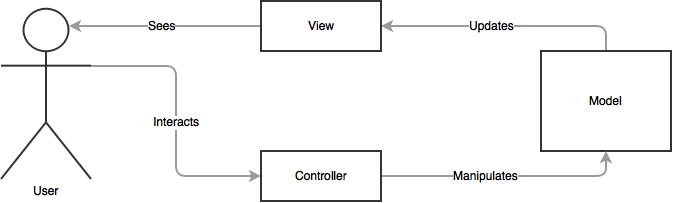
\includegraphics[width=1.0\textwidth]{images/mvc}
  \caption{Information Exchange in an MVC Application.} \label{fig:MVC} 
\end{figure}

Laravel, an open-source PHP web application framework intended for the development of web applications following the MVC architectural pattern, developed by Taylor Otwell, was chosen after researching various frameworks \cite{Laravel:Home}. Laravel was chosen over other frameworks for a number of reasons. Not only does it provide an implementation of the MVC pattern, but it also allows allows the user to define custom routes and decide where each route leads rather than having the URL be determined by the file path. Additionally, Laravel comes with solutions to a lot of common tasks and problems straight out of the box making it easier to develop the system straight away without having to ``reinvent the wheel''.

\paragraph{jQuery} jQuery is a fast, small, and feature-rich JavaScript library \cite{jQuery:Home}. It will be used over standard JavaScript as it makes things like HTML document traversal and manipulation, event handling, animation, and Ajax much simpler with an easy-to-use API that works across a multitude of browsers \cite{jQuery:Home}. Although jQuery doesn't necessarily provide any additional functionality over JavaScript as it is powered by JavaScript, it provides shorter notations for common JavaScript functions and provides implementation of features that are lacking in JavaScript, or take long to implement. It can be setup and used by simply including a single script in the document.

\paragraph{Bootstrap} Bootstrap is the most popular HTML, CSS, and JS framework for developing responsive, mobile first projects on the web \cite{Bootstrap:Home}. The main advantage of using Bootstrap is that it easily and efficiently scales your websites and applications with a single code base, from phones to tablets to desktops with CSS media queries. Additionally Bootstrap comes with a whole range of HTML, CSS and jQuery components, that have been pre-styled, further speeding up the development process.

\subsubsection{Storage}
One of the most fundamental parts of the system is retaining the data that the users enter into the system. There are two different storage solutions for storing and querying the data provided by users. These are both discussed below.

\paragraph{MySQL} MySQL is an open source database management system used for managing data held in a relational database management system (RDBMS) \cite{MySQL:Home}. An SQL database will be used to store all textual information entered by the users. This includes user information, location data, item details and any other necessary information. SQL databases are not encrypted and hence any user credentials such as password will be stored in an encrypted format to prevent access to user accounts in case of a breach.

\paragraph{Resources}
Along with textual input, it is also necessary to store the files associated as resources with items, uploaded by the users. One approach to this could be to convert the file to binary and store the binary data in the SQL database. However this approach would lead to the database rapidly growing in size and in turn affecting the performance. Not only would queries take longer to execute but also increase page load times due to the large record sizes. Another approach would be to store any uploaded files either on a storage server or on the web server so they are available on demand. This would result in faster loading time for pages containing these resources as they do not have to be transferred over the network. Due to this, the latter approach will be used during development.

\subsubsection{Third Party APIs}

\paragraph{Geocoding and Reverse Geocoding} Google Maps provides a GeoCoding API which allows converting of addresses (like ”1600 Amphitheatre Parkway, Mountain View, CA”) into geographic coordinates (like latitude 37.423021 and longitude -122.083739) \cite{Google:GeoCoding}. As users will enter addresses, which have an inconsistent format, the GeoCoding API will be used to translate these addresses to coordinates, which have a consistent format, so that they can be stored in a database. The API can also be used in reverse to translate coordinates into addresses, which will be necessary when displaying location data to users.

\paragraph{Google Maps} Google provides a JavaScript API for their maps service. The API allows the developer to build a custom map for their site using styled maps, 3D buildings, indoor floor plans, multi-modal directions and more \cite{Google:Maps}. Interactive maps help the users to visualise the data as well as making it easier to navigate the data. Overall, this leads to a better a user experience and provides a better system. The API will be used with the coordinates obtained from the Police API or items reported as stolen to place markers on a visual map in order to help locate stolen items. In addition to this, the maps API can also be used to highlight locations where an item may have been spotted and provide directions for relocation.

\paragraph{Metropolitan Police API}
Although the inclusion of this API and feature does not impact the core functionality of the system, it does raise awareness of the issue the system is trying to tackle which may encourage users to register on and use the system. The API is implemented as a standard JSON web service using HTTP GET and POST requests and provides a rich data source for information such as street-level crime and outcome data \cite{Police:API}. This data can be used along with the Google Maps API to plot a map of all the crimes around the user and will be included in the system.

\newpage